\documentclass[notes,page number]{beamer}

%\usecolortheme{crane}
\mode<presentation>
{
 \usetheme{Singapore} %
}
 %\usepackage{beamerthemesplit}
\usepackage{beamerfontthemeprofessionalfonts}
\usepackage{fancyhdr, epsfig, psfrag}
\usepackage{beamerthemeshadow}
\setbeamertemplate{navigation symbols}{}
\usepackage[english]{babel}

\usepackage{bbm}
%\usepackage{pstricks,pst-grad,pst-node}

\usepackage{tikz}
\usetikzlibrary{shadows,positioning}
\title{Verified Security of Hashed Authenticated Key-Exchange Protocols} 
\subtitle{Work in progress}
\author{
  G. Barthe\inst{1}
  \and
  J. M. Crespo\inst{1}
  \and
  C. Ene\inst{2}
  \and 
  C. Kunz\inst{1}
  \and\\
  Y. Lakhnech\inst{2}
  \and
  B. Gregoire\inst{3}
  \and
   S. Zanella B\'eguelin\inst{4}
}
\institute{\inst{1} IMDEA Software, Madrid, Spain \\
  \inst{2}University of Grenoble, CNRS - VERIMAG, France\\
\inst{3} INRIA, Sophia-Antipolis\\
\inst{4} MSR, Cambridge, UK}
\date{FCC 2012}

\newcommand\NAXOS{\textsc{Naxos}}
%\newcommand\vec[1]{\overrightarrow{#1}}
\newcommand\Axiom{\mathbf{Axiom}}
\newcommand{\EasyCrypt}{\textsf{EasyCrypt}}
\newcommand{\Equiv}[4]{\vDash {#1} \sim {#2} : {#3} \Rightarrow {#4}}
\newcommand{\Pre}{\Psi}
\newcommand{\Post}{\Phi}
\newcommand{\Inv}{\Phi}
\newcommand{\side}[1]{\langle #1 \rangle}
\newcommand{\sidel}{\side{1}}
\newcommand{\sider}{\side{2}}
\newcommand{\eqobsin}{\mathsf{eqobs\_in}}
\newcommand{\eqobsout}{\mathsf{eqobs\_out}}


\newcommand{\psc}{b}
\newcommand{\esc}{e}
\newcommand{\ssc}{s}
\newcommand{\essc}{es}

\newcommand\inpmess{\mathsf{init}}
\newcommand\respmess{\mathsf{resp}}
\newcommand\priv{\mathsf{pv}}

\newcommand\Eph{\mathsf{EphK}}
\newcommand\Pv{\mathsf{PvK}}
\newcommand{\bsy}{m_B}
\newcommand{\bsx}{m_A}
\newcommand{\hlist}{L_{\mathbf{H}}}
\newcommand{\slist}{L_{{\sc ss}}}

\newcommand\AC{\textsf{AC}}

\newcommand\GROM{\textsc{GROM}}
\newcommand\hmqv{\ensuremath{\mathsf{HMQV}}\xspace}
\newcommand\mqv{\ensuremath{\mathsf{MQV}}\xspace}
\newcommand\naxos{\ensuremath{\mathsf{NAXOS}}\xspace}
\newcommand\keap{\ensuremath{\mathsf{KEA+}}\xspace}

\newcommand\Hyp{\ensuremath{\mathcal{H}}}

\newcommand\Gammat{\Gamma^T}
\newcommand\Mo{\textsf{M}}

\newcommand\natf{\nat_{n_f}}
\newcommand\natg{\nat_{n_g}}
\newcommand\pub{\textsf{pub}}
\newcommand\Pub{\textsf{Pub}}
\newcommand\chal{\textsf{chal}}
\newcommand\Chal{\textsf{Chal}}
\newcommand\Find{\textsf{Find}}
\newcommand\dist{\textsf{dist}}
\newcommand\stopp{\textsf{stop}}
\newcommand\vo{\textsf{v}}
\newcommand\oo{\textsf{o}}
\newcommand\last{\mbox{last}}
\newcommand\lastm{\mbox{lastM}}
\newcommand\lasts{\mbox{lastS}}
\newcommand\lastv{\mbox{lastV}}
\newcommand\firstm{\mbox{firstM}}
\newcommand\firsts{\mbox{firstS}}
\newcommand\firstv{\mbox{firstV}}
\newcommand\ev{\textsf{Ev}}
\newcommand\obs{\textsf{obs}}
%\newcommand\trace{\cT}
\newcommand\Exec{\mathsf{Exec}}
\newcommand\Execf{\mathsf{Exec}_f}
\newcommand\Execg{\mathsf{Exec}_g}
\newcommand\trace{\mathsf{trace}}
\newcommand\Traces{\mathsf{Traces}}
\newcommand\IT{\mathsf{IT}}
\newcommand\blue[1]{{\color{blue}{#1}}}
\newcommand\red[1]{{\color{red}{#1}}}
\newcommand\rel[2]{\mathcal{R}^{#1}_{#2}}
%\renewcommand\afr{\textsf{fr}}

%\theoremstyle{definition}

%%%%%%%%%%%%%%%%%%%%%%%%%%%%%%%%%%%%%%%%%%

\newenvironment{nb}[1][N.B.]{\begin{trivlist}
 \item[\hskip \labelsep {\bfseries #1}]\bf }{\hfill
   $\Box$\end{trivlist}}
\newenvironment{remark}[1][Remark]{\begin{trivlist}
 \item[\hskip \labelsep {\bfseries #1}] }{\hfill $\Box$\end{trivlist}}

%%%%%%%%%%%%%%%%%%%%%%%%%%%%%%%%%%%%%%%%%%%%%%555
\newcommand\cinp{cin}
\newcommand\cout{cout}
\newcommand\CQ{cQ}
\newcommand\cOC{\textsf{CO}}
\newcommand\cOCin{\textsf{COin}}
\newcommand\cOCout{\textsf{COout}}
\newcommand\MemC{\textsf{MC}}
\newcommand\cdi{\textsf{d}^I_{\cC}}
\newcommand\cm{cm}


\newcommand\cpub{\textsf{cpub}}
\newcommand\CPub{\textsf{CPub}}
\newcommand\Part{\textsf{Part}}
\newcommand\cfind{\textsf{cfind}}
\newcommand\CFind{\textsf{CFind}}
\newcommand\cchal{\textsf{cchal}}
\newcommand\CChal{\textsf{CChal}}
\newcommand\cres{\textsf{cres}}
\newcommand\CRes{\textsf{CRes}}
\newcommand\SA{S^\cA}
\newcommand\TA{\cA_t}
\newcommand\ct{T}
\newcommand\FA{\cA_f}
\newcommand\GA{\cA_g}

\newcommand\StA{St}

\newcommand\TS{\textsc{Ts}}
\newcommand{\given}{\rightarrow}


\newcommand\cO{\mbox{\textsf{O}}}
\newcommand\cOf{\textsf{Of}}
\newcommand\cOg{\textsf{Og}}
\newcommand\OL{\mbox{\textsf{Ol}}}
\newcommand\Mem{\mbox{\textsf{M}}}
\newcommand\di{\textsf{d}^I}
\newcommand\In{\mbox{\textsf{In}}}

%\newcommand\cOC{\mbox{\textsf{CO}}}
\newcommand\CQue{\mbox{\textsf{CQue}}}
\newcommand\CIn{\mbox{\textsf{CIn}}}
\newcommand\COut{\mbox{\textsf{Cout}}}
\newcommand\Out{\mbox{\textsf{Out}}}
\newcommand\Inf{\mbox{\textsf{FIn}}}
\newcommand\Outf{\mbox{\textsf{GOut}}}
\newcommand\Ing{\mbox{\textsf{GIn}}}
\newcommand\Outg{\mbox{\textsf{GOut}}}
\newcommand\Sys{\mbox{\textcursive{S}}}
\newcommand\Cframe{\textbf{\cal F}}
%\newcommand\Sys{\textsf{S}}
\newcommand\Res{\mbox{\textsf{Res}}}
\newcommand\ol{\textsf{ol}}
\newcommand\Que{\textsf{Que}}
%\newcommand\inp{\textsf{in}}
\newcommand\out{{out}}
\newcommand\inp{in}

\newcommand\Q{Q}
\newcommand\AQ{\out}
\newcommand\oaep{\textsf{oaep}}
\newcommand\Ask{\textsc{Ask}}
\newcommand\cH{\mathcal{H}}
\newcommand{\boxedeqn}[1]{%
  \[\fbox{%
      \addtolength{\linewidth}{-2\fboxsep}%
      \addtolength{\linewidth}{-2\fboxrule}%
      \begin{minipage}{\linewidth}%
      \begin{equation}#1\end{equation}%
      \end{minipage}%
    }\]%
}
\newcommand\pad{\mbox{pad}}
\newcommand\post{\textsf{pst}}
\newcommand\inv{\textsf{inv}}
\newcommand\comment[1]{}
\newcommand\Sdet{\textsc{Sd}}
\newcommand{\List}{\mathsf{List}}
\newcommand\Win{\textsc{Win}}
\newcommand\Winfdh{\textsc{Win}}
\newcommand\Ou{\;\mbox{or}\;}

\newcommand{\game}[2]{\langle #1 \!\! \parallel\!\! #2\rangle}
\newcommand{\gamef}[2]{\langle #2 \!\! \parallel \!\! #1\rangle_f}
\newcommand{\gameg}[2]{\langle #2 \!\! \parallel \!\! #1\rangle_g}
\newcommand{\gameo}[3]{\langle #1 \!\! \mid \!\! #3 \!\! \parallel
  \!\! #2\rangle}
\newcommand{\gameoo}[3]{\langle #1 \!\! \mid \!\! #3 /\cO \!\! \parallel
  \!\! #2\rangle} 
\newcommand{\gamefk}[3]{\langle #2 \!\! \parallel \!\! #1\rangle^{#3}_f}
\newcommand{\gamegk}[3]{\langle #2 \!\! \parallel \!\! #1\rangle^{#3}_g}

\newcommand{\sres}{r}
\newcommand{\round}[3]{\mathbf{R}_{#1\parallel #2}^{#3}}
\newcommand{\ctxt}{\mathbf{c}}
\newcommand{\frd}{{\sf smp}}
\newcommand{\fco}{{\sf co}}
\newcommand{\adistr}{d}
\newcommand{\unel}{!}

\newcommand{\Imm}{\mathbb{I}}
\newcommand{\I}{{\cal I}}

\newcommand{\succow}{\textbf{SuccOW}}

%%%%%%%%%Oracles%%%%%%%%%%%%%%%%%%%%%%%%%%%%%%%%%%%%%%%%%%%%%%%%%%%%%%%%%%%%%%%%%
\newcommand{\Honest}{\mathbf{Hon}}
\newcommand{\Corrupt}{\mathbf{Cor}}
\newcommand{\SessionKeyReveal}{\mathbf{KeyR}}
\newcommand{\Test}{\mathbf{Test}}
\newcommand{\SessionRandomReveal}{\mathbf{EphR}}
\newcommand{\SessionStateReveal}{\mathbf{StaR}}
\newcommand{\Register}{\mathbf{Reg}}
\newcommand{\GapSessionString}{\mathbf{GSS}}
\newcommand{\SessionString}{\mathbf{SS}}
\newcommand{\RandomReveal}{\mathbf{RR}}
\newcommand{\AllReveal}{\mathbf{AR}}
\newcommand{\Init}{\mathbf{Init}}
\newcommand{\Comp}{\mathbf{Comp}}
\newcommand{\Resp}{\mathbf{Resp}}
\newcommand{\SecK}{\mathbf{SecK}}
\newcommand{\EqS}{\mathbf{EqS}}
\newcommand{\SameSeS}{\mathbf{SameSeS}}

%%%%%%%%%%%%%%%%%%ss-game   %%%%%%%%%%%%%%%%%%%%%%%%%%%%%%%%%%%%%%%%%%%%%%%%%%%%%%%%%%
%\newcommand{\Hyp}{\mathbf{Hyp}}
\newcommand{\x}{\mathbf{x}}
\newcommand{\y}{\mathbf{y}}
\newcommand{\w}{\mathbf{w}}
\newcommand{\z}{\mathbf{z}}


%%%%%%%%%%%%%%%%%%%%%%%%%%%%%%%%%%%%%%%%%%%%%%%%%%%%%%%%%%%%%%%%%%%%%%%%%%%%%%%%%%

\newcommand{\fstp}[1]{{[#1]_1}} 
\newcommand{\zq}{\mathbb{Z}_q}
\newcommand{\oinp}{\Lambda}
\newcommand{\oout}{\Omega}
\newcommand{\ainp}{{\cal V}}
\newcommand{\aout}{{\cal R}}
\newcommand{\coi}{\Theta}
\newcommand{\gout}{{\cal T}}
\newcommand{\ismp}{{\cal X}}
\newcommand{\ad}{\mathbb{A}}
\newcommand{\fr}{\mathbb{F}}
\newcommand{\afr}{s}
\newcommand{\synframe}{s}
\newcommand{\semframe}[1]{\langle #1\rangle}
\newcommand{\semf}[1]{\langle\!\langle #1\rangle\!\rangle}
\newcommand\pss{\textsc{\bf PSS}}
\newcommand\fdh{\textsc{\bf FDH}}
\newcommand\Frame[1]{{\bf \pss#1}}
\newcommand\Oaep[1]{{\bf OAEP#1}}
\newcommand\NegUNIV{\textbf{(NegUNIV)}}
\newcommand\false{\textsf{false}}
%commands for oracles implementations:
\newcommand\sig{\mathsf{sig}}
\newcommand\Sig{{\cal S}}
\newcommand{\si}{\mbox{if }}
\newcommand{\alors}{\mbox{ then }}
\newcommand{\sinon}{\mbox{else }}
\newcommand{\rep}{\mbox{return }}
\newcommand{\soit}{\mbox{let }}
\newcommand{\finsi}{\mbox{ fi}}
\newcommand{\find}{\mbox{find }}
\newcommand{\st}{\mbox{ such that }}
\newcommand{\sampled}{\stackrel{\small{\$}}{\leftarrow}}
\newcommand\as[2]{#1\!\stackrel{\small{\$}}{\leftarrow}\! #2}
\newcommand{\A}{\mathbf{A}}
\newcommand{\B}{\mathbf{B}}
\newcommand{\aP}{\mathbf{P}}

\newcommand{\zo}{{[0,1]}}
\newcommand{\cfr}{\bar{v}}
\newcommand{\gindcpa}{{\sf G}^{\mathrm{cpa}}}

\newcommand{\State}{{\cal S}}

\newcommand\ROM{\textsc{ROM}}
\newcommand\s{\textsc{ses}}
\newcommand\sk{\textsc{sk}}
\newcommand\pk{\textsc{pk}}

%\newcommand\ska{a}
%\newcommand\pk_a{A}
%\newcommand\sk_b{b}
%\newcommand\pk_b{B}



\newcommand{\kgen}{{\cal KG}}
\newcommand{\enc}{{\cal E}}

\newcommand{\unid}{{\cal U}}
%\newcommand{\bool}{\mathsf{Bool}}
\newcommand{\unidbool}{\unid_{\bool}}
\newcommand{\zp}{\mathbb{Z}_p}

\newcommand{\tnu}[3]{{#1}\stackrel{r}{\leftarrow}{#2},~ #3}
\newcommand{\unu}[2]{{#1}\stackrel{r}{\leftarrow}{U},~ #2}
\newcommand{\sspace}{S_{{\sf rnd}}}
\newcommand{\sorts}{S}
\newcommand{\symb}{F}


%\newcommand{\fv}{{\sf fv}}
\newcommand{\wth}[2]{[#2/#1]}

\newcommand{\aterm}{t}
\newcommand{\asort}{\sigma}
\newcommand{\bsort}{\tau}
\newcommand{\atheory}{E}
\newcommand{\asym}{f}
\newcommand{\aalg}{{\cal A}}
\newcommand{\acarr}{A}

%\newcommand{\turn}[1]{\vdash #1}
\newcommand{\turnae}[1]{ \vdash #1}
\newcommand{\peturnae}[1]{ \Vdash_{\atheory} #1}

\newcommand{\infr}[2]{\textstyle \frac{\stackrel{\textstyle #1}{}}{\stackrel{}{\textstyle #2}}}


\newcommand{\bits}{{\sf Bits}}
%\newcommand{\bs}[1]{{\sf BS}^{#1}}
%\newcommand{\xor}{\oplus}
\newcommand{\concat}{|}
\newcommand{\pproj}{\pi}
\newcommand{\lproj}{\overline{\pi}}
\newcommand{\rproj}{\overline{\pi}}


%\newcommand{\sem}[2]{[\!\![ #1 ]\!\!]_{#2}}

%\newcommand{\alarm}[1]{\marginpar{{\tiny #1}}}
\newcommand{\tcomment}[1]{{\sf Comment: #1}}



%%%%%%%%%%%%%%%%%%%%%%%%%%%%%%55

\newcommand\Inter{\textsc{I}}
\newcommand\cI{\mathcal{I}}
\newcommand{\bs}[1]{\{0,1\}^{#1}}
\newcommand\cS{\mathcal{S}}
\newcommand\FDH{\textsf{FDH}}
%\newcommand\OW{\textsf{OW}}

\newcommand\bv{\textsf{bv}}
\newcommand\fv{\textsf{fv}}
\newcommand\com[1]{\framebox{\textbf{#1}}}
 \newcommand{\comm}[1]{}

\newcommand{\TODO}[1]{[\textbf{TODO} : #1]}
\newcommand\xor\oplus
\newcommand\Dist{{\cal D}}
\newcommand{\distr}[1]{\Dist (#1)}
\newcommand{\darrow}[1]{\stackrel{\Dist}{\rightarrow}(#1)}
\newcommand{\darrownb}[1]{\stackrel{\Dist}{\rightarrow}#1}
\newcommand{\darrowws}[2]{\stackrel{\Dist_{#2}}{\longrightarrow}#1}

\newcommand\DistG{\Dist(\Gamma,\vH,\cF)}
\newcommand{\DistGen}{\overline{\Dist}}
\newcommand{\DistGenG}{\DistGen(\Gamma,\vH,\cF)}
\newcommand\cD{\mathcal{D}}
\newcommand\cdis{\mathcal{D}}
\newcommand\cM{\mathcal{M}}
\newcommand\cU{\mathcal{U}}
\newcommand\cX{\mathcal{X}}
\newcommand\cY{\mathcal{Y}}
\newcommand\cZ{\mathcal{Z}}
\newcommand\cV{\mathcal{V}}
\newcommand\cJ{\mathcal{J}}

\newcommand\M{\textbf{M}}
\newcommand\D{\textbf{D}}
\newcommand\E{\textbf{E}}
\newcommand\F{\textbf{F}}
\newcommand\R{\textbf{R}}
\newcommand\C{\textbf{C}}
\newcommand\sem[1]{\ensuremath{[\![#1]\!]}}
\newcommand\sema[1]{\ensuremath{[\![#1]\!]^{\#}}}
%\newcommand\cP{\mathcal{P}}
\newcommand\cT{\mathcal{T}}
\newcommand\cF{\mathbbm{F}}
\newcommand\cR{\mathcal{R}}
\newcommand\lfp{\textit{lfp}}
\newcommand\astate[1]{S_{#1}^{\#}}
\newcommand\base{\textsf{B}}
\newcommand\return{\textsf{return}}
\newcommand\error{\emph{"error"}}
\newcommand\abort{\textsf{abort}}
\newcommand\nat{\mathbbm{N}}
\newcommand\integer{\mathbbm{Z}}
\newcommand\real{\mathbbm{R}}
\newcommand\bool{\mathbbm{B}}
\newcommand\Adv{\textsf{Adv}}
\newcommand\pa{\textsf{pa}}
\newcommand\opr{\overline{\textsf{Pr}}}
\newcommand\test{\textsf{test}}
\newcommand\Succ{\textsf{Succ}}
\newcommand\Ext{\textsf{Ext}}

\newcommand\lrulet[3]{\infer[#1]{#3}{#2}}

\newcommand{\Exp}{\textbf{Exp}}
\newcommand{\hH}{\textbf{H}}
\newcommand{\fvar}{\textsf{fvar}}
\newcommand{\favar}{\textsf{favar}}
\newcommand{\AVar}{\textsf{AVar}}
%\newcommand{\Var}{\textsf{Var}}
\newcommand\aA{\textsf{A}}
%\newcommand{\sem}[1]{\ensuremath{[\![#1]\!]}}


\newcommand\vH{\vec{H}}
\newcommand{\vHp}{\vec{H'}}
\newcommand{\vHdp}{\vec{H''}}

\newcommand\true{\textsf{true}}
\newcommand\GE{{G\!E}}
\newcommand\name{\mathcal{N}}
\newcommand\cpa{cpa}
\newcommand\cca{cca}
\newcommand\ind{ind}
\newcommand\indcpa{{\sf IND-CPA}\xspace}

\newcommand\kPk{\textsf{Pk}}
\newcommand\kSk{\textsf{Sk}}
%\newcommand\max{\textsf{max}}
\newcommand\inferprime[2]{\infer{#2}{#1}}
\newcommand\oute{\mbox{out}_e}
\newcommand\ine{\mbox{in}_e}
\newcommand\outde{\mbox{out}_d}
\newcommand\inde{\mbox{in}_d}
%%%%%%%%%%%%%%%%%%%%%%%%%%%%%%%%%%%%%%%%%%
%\newcommand\D{\textsf{D}}
\newcommand\Var{\textsf{Var}}
\newcommand\var{\textsf{var}}
\newcommand\cmd{\textsf{c}}
\newcommand\acmd{\textsf{ac}}
\newcommand\scmd{\textsf{sc}}
\newcommand\decl{\textsf{decl}}
\newcommand\prog{\textsf{prog}}
\newcommand\call{\textsf{call}}
%\newcommand\pk{\textit{pk}}
%\newcommand\sk{\textit{sk}}
\newcommand\ras[1]{\randd{#1}{\mathcal{U}}}
\newcommand\owas[3]{#2:=#1(#3)}%{\textsf{Ow}(#1,#2,#3)}
\newcommand\owpas[3]{#2:=#1(#3)}
\newcommand\hashas[3]{#2:=#1(#3)}%{\textsf{Hash}(#1,#2,#3)}
\newcommand\Pkey{\textsf{PKey}}
\newcommand\Skey{\textsf{SKey}}
%%%%%%%%%%%%% sets of functions %%%%%%%%%%%%%%%%%%%%%%%%
\newcommand\OW{\ensuremath{\mathcal{O}}}
\newcommand\OWP{\ensuremath{\Pi}}
\newcommand\HASH{\ensuremath{\mathcal{H}}}
\newcommand\Pk{\textsf{Pk}}
\newcommand\Sk{\textsf{Sk}}
%%%%%%%%%%%%%%%%%%%%%%%%%%%%%%%%%%%%%
\newcommand\Ow{\mathbbm{O}}
\newcommand\T{\mathbbm{T}}
%%%%%%%%%%%%%%%%%%%%%%%%%%%%%%%%%%%%%%%%%%%%%%%%%%%
\newcommand\PH{\textsf{P}}
\newcommand\SH{\textsf{S}}
\newcommand\Int{\textsf{I}}
%%%%%%%%%%%%%%%%%%%%%%%%%%%%%%%%%%%%%%%%%%%%%%%%%%%
\newcommand\ow{f}
\newcommand\Io{\textsf{I}_{\textsf{o}}}
\newcommand\DoH[2]{\textsf{H}(#1,#2)}
\newcommand\DoOW[1]{\mathcal{O}(#1)}
\newcommand\dom{\textsf{dom}}
\newcommand\range{\textsf{rng}}
\newcommand\res{\textsf{res}}
\newcommand\ares{\textsc{r}}
\newcommand\achal{\textsc{c}}
\newcommand\WS{\textsf{WS}}
\newcommand\Indis{\textsf{Indis}}
\newcommand\WIndis{\textsf{WIndis}}
\newcommand\randd[2]{{#1}\!\leftarrow\! {#2}}
\newcommand{\assign}[2]{{#1}\!\leftarrow\!{#2}}
\newcommand\pr{\textsc{Pr}}
\newcommand\ipr{\textsc{P}^I}
\newcommand\tpr{\textsc{P}^T}
\newcommand\fpr{\textsc{P}^L}

\newcommand\Lw{\textsf{P}}
\newcommand\Hg{\textsf{S}}

\newcommand\cE{\mathcal{E}}
\newcommand\cK{\mathcal{K}}
\newcommand\cG{\mathcal{G}}
%\newcommand\cA{\mathcal{A}}
%\newcommand\cB{\mathcal{B}}
\newcommand\pA{\ensuremath{{A}}}
\newcommand\pB{\ensuremath{{B}}}
\newcommand\sA{\ensuremath{a}}
\newcommand\sB{\ensuremath{b}}
\newcommand\pC{\ensuremath{\hat{C}}}
\newcommand\pD{\ensuremath{\hat{D}}}
\newcommand\cA{\ensuremath{\hat{A}}}
\newcommand\cB{\ensuremath{\hat{B}}}
\newcommand\cC{\ensuremath{\hat{C}}}
\newcommand\cP{\ensuremath{\hat{P}}}

%\newcommand\cT{\mathcal{T}}
\newcommand\ecT[1]{(\mathcal{T}_{\eta}(#1))_{\eta\in \nat}}

\newcommand\sid{\ensuremath{\textsc{sid}}}

% \newcommand{\qed}{\nobreak \ifvmode \relax \else
%       \ifdim\lastskip<1.5em \hskip-\lastskip
%       \hskip1.5em plus0em minus0.5em \fi \nobreak
%       \vrule height0.75em width0.5em depth0.25em\fi}
\newcommand{\oracle}{\mathcal{O}}
\newcommand{\V}[1]{\overrightarrow{#1}}

\newcommand{\upd}[2]{#1 + #2}
\newcommand{\updv}[2]{#1 + #2}
% \bindH{H}{y}{x}
\newcommand{\bindH}[3]{\{\T_{#1} \mapsto (#2,#3)\}}
% \rebindH{\vH}{H}{y}{x}
\newcommand{\rebindH}[4]{\updv{#1}{\bindH{#2}{#3}{#4}}}
%
\newcommand{\zero}[1]{\textsf{zero}_{#1}}
%\newcommand{\log}{\textsf{log}}
\newcommand{\invf}{f^{-1}}
\newcommand{\Hetc}[1]{{(#1,\vH,(f,\invf))}}
\newcommand{\Hpetc}[1]{{(#1,\vHp,(f,\invf))}}
\newcommand{\vHf}{{\vH,f}}
\newcommand{\rebind}[3]{\mbox{\textsf{rebind}}_{#1}^{#2\mapsto #3}}
\newcommand{\iffdef}{\iff_{\mbox{def}}}

\newcommand{\ret}{\mbox{ret}}
\newcommand{\OR}{\mbox{\textrm{onlyreads}}}
\newcommand{\ws}{\mbox{ws}}
\newcommand{\strs}{\mbox{ss}}
%%%%%%%%%%%%%%%%%%%%%%%%%%%%%%%%%
%macros ajout�es pour les conditionnels et les frames 
\newcommand\FV{\mathcal{F}}  % function variables
%\newcommand\cT{\mathcal{T}}  %  terms (d�j� �crit)
\newcommand\probterm{\mathcal{PT}} %  probabilistic terms
\newcommand\draw[2]{\mbox{\texttt{let}\ensuremath{\: \randd{#1}{#2}} 
\texttt{in}}}
\newcommand\p{\bold p}
\newcommand\word[1]{\ensuremath{ \{0,1\}^{#1(\eta)} }}
\newcommand\Let{\texttt{let}}
%qd y a qu'un machin a mettre
\newcommand\letvert[1]{\begin{pmatrix} #1 \end{pmatrix} \ \! \cdot} 
 %nb : il faut remplacer #1 par les tirages \randd{}{} en les s�parant par \\
% pb au dessus de 10 lignes 

\newcommand\littleletvert[1]{\footnotesize \Let \begin{pmatrix} #1 \end{pmatrix} \ \! 
\mbox{\texttt{in}} \normalsize} 
% pareil en petit pour que �a tienne
\newcommand{\TO}{{\cal TO}}
\newcommand{\TI}{{\cal TI}}

\newcommand{\nn}{:} %negligible
\newtheorem{axiom}{Axiom}

\newcommand\Plaintext{\textsf{PT}}
\newcommand\Ciphertext{\textsf{CT}}
\newcommand\SP{\hbox{\hskip 1.1pt$\Diamond$\hskip -4.8pt-\hskip 3.8pt}}
\newcommand\AP{\hbox{\hskip 1.1pt$\Box$\hskip -4.8pt-\hskip 3.8pt}}
\newcommand\Before{\textbf{\;B\;}}
\newcommand\query{\mathcal R}

\newcommand\fram{\textsf{Fr}}

\newcommand\Bad{\textsf{Bad}}
\newcommand\pow{\textsf{pow}}
\newcommand\until{\mathcal{U}}

\newcommand\nO{\mathcal{O}ut}
\newcommand\nI{\mathcal{I}n}

%%% Local Variables: 
%%% mode: latex
%%% TeX-master: "main"
%%% End: 


\begin{document}
\begin{frame}
\titlepage
\end{frame}
%\section{Introduction}
\begin{frame}
  \frametitle{Key Exchange Protocols}
A pool of $n$ participants try to establish a comon symmetric session key, in the presence of an adversary.
\begin{tikzpicture}
\node (n1) {
\includegraphics[width=0.3\textwidth]{alice.pdf}};
\node (n2) [right= of n1] {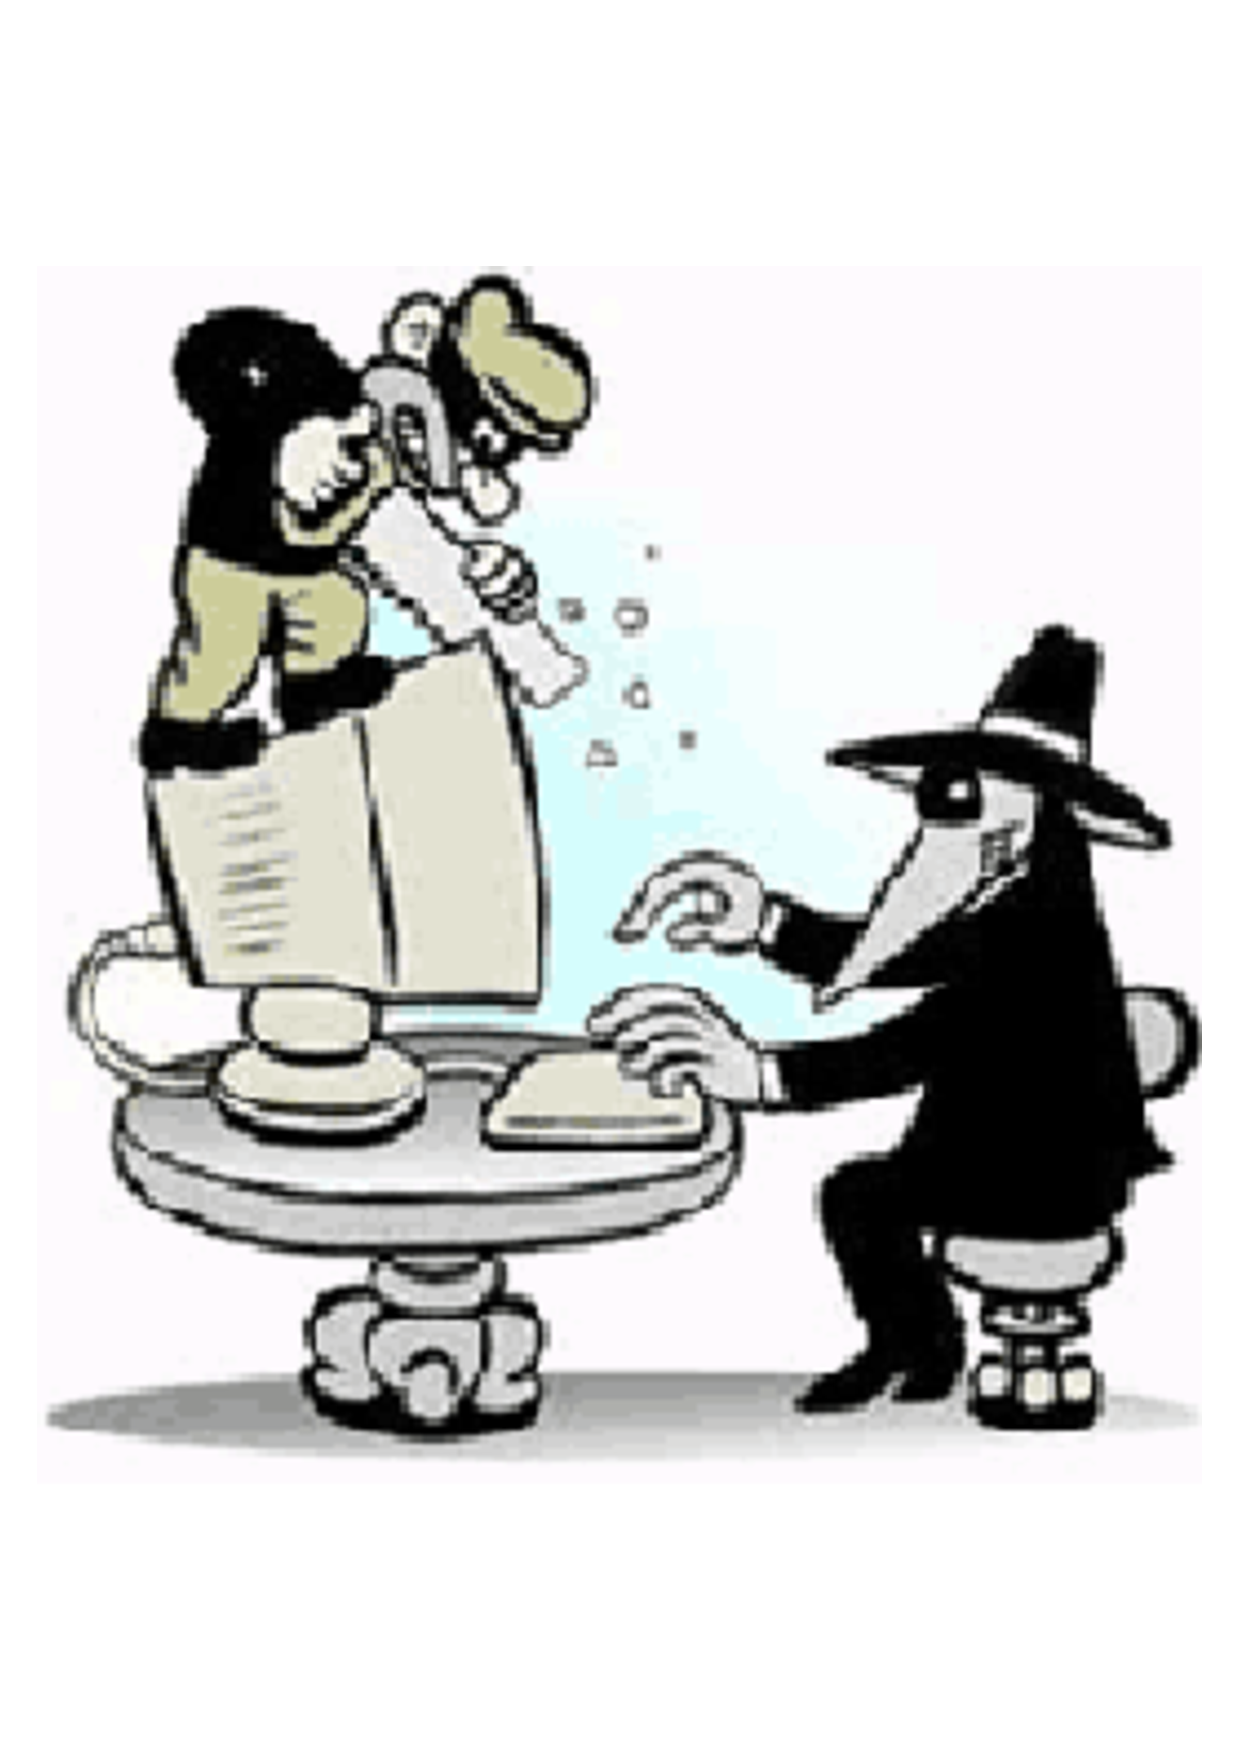
\includegraphics[width=0.3\textwidth]{spy.pdf}}edge[thin, <-] node[] {} (n1);

\node (n3) [right= of n2] {
\includegraphics[width=0.3\textwidth]{bob.pdf}} edge[thin, <-] node[] {} (n2);



\end{tikzpicture}

\end{frame}
\begin{frame}
  \frametitle{Security Goals}
  \begin{block}{Definition (Key privacy)}
No one except the legitimate parties can distinguish the established key from a random key.
  \end{block}
\begin{block}{Definition (implicit key authentication)}
In presence of a passive adversary, two legitimate parties engaged in
a session, will compute the same key.
\end{block}
Not to be confused with key confirmation: no one can make a legitimate
partner believe he shares a key with a partner, unless this is the
case.
\end{frame}
\begin{frame}
  \frametitle{Diffie-Hellman}
\begin{figure}
\begin{displaymath}
\begin{array}{c@{}c@{}c} A&&B\\
\begin{array}[m]{c}
x\xleftarrow{\$}\mathbb{Z}_q\\[5ex]
\end{array}
&
\begin{array}[m]{c}
\begin{tikzpicture}
\node (n1) {};
\node (n2) [right=120pt of n1] {}
 edge[thick,<-] node[yshift=7pt]
 {$A, X=g^{x}$} (n1);
\node (n1') [below= 15pt of n1] {};
\node (n2') [right=120pt of n1'] {$y\xleftarrow{\$}\mathbb{Z}_q$}
 edge[thick,->] node[yshift=7pt]
 {$B, Y=g^{y}$} (n1');
\end{tikzpicture}
\end{array}
\end{array}
\end{displaymath}
\end{figure}
\end{frame}
\begin{frame}
  \frametitle{Hashed DH-based key Exchange Protocols}
  \begin{itemize}
  \item Participants exchange messages that allow each party to compute at the end of a session a bitstring, called \emph{session string}.
  \item The session key is derived from the session string by applying a hash function.
  \end{itemize}
Two types of protocols :
  \begin{itemize}
  \item the flow of messages is that of DH;
    it is the way the session string is
    computed that guarantees authentication. May suppose public keys, or
    symmetric keys,... . Matsumoto, Takashima and Imai'86
  \item the flow of messages is modified
    modified, e.g., by adding signatures, encryptions, further rounds,.... Bellovin and Merrit'92
  \end{itemize}
\end{frame}
%% \begin{frame}
%%   \frametitle{Basic Authenticated Diffie-Hellman}
%% \begin{figure}
%% \begin{displaymath}
%% \begin{tikzpicture}
%% \node (n0){$A$};
%% \node (n0') [right=140 pt of n0] {$B$};
%% \node (n1) [below=15 pt of n0] {};
%% \node (n1') [below= 15pt of n0'] {};
%% \node (n2) [right=0 pt of n1] {$x\xleftarrow{\$}\mathbb{Z}_q$} edge[thick, ->] node[yshift=7pt]{$A, X=g^{x}$}(n1');
%% \node (n3) [below=15pt of n2] {};
%% \node (n3')[right=10pt of n3]{};
%% \node (n2') [right=130 pt of n3] {$y\xleftarrow{\$}\mathbb{Z}_q$}
%%  edge[thick,->] node[yshift=10pt]
%%  {$B, Y=g^{y}, \sig_B(X,Y)$} (n3');
%% \node (n4) [below=15pt of n3]{};
%% \node (n5) [right=10pt of n4]{};
%% \node (n4') [right= 130pt of n4] {}
%%  edge[thick,<-] node[yshift=7pt]
%%  {$\sig_A(Y,g^{x})$}(n5);

%% \end{tikzpicture}
%% \end{displaymath}
%% \end{figure}
%% \end{frame}
\begin{frame}
  \frametitle{HMQV}
A variant of MQV.

\[\pA=g^a,\;\pB=g^b\]
\begin{figure}
\begin{displaymath}
\begin{array}{c@{}c@{}c} A&&B\\
\begin{array}[m]{c}
x\xleftarrow{\$}\mathbb{Z}_q\\[5ex]
\end{array}
&
\begin{array}[m]{c}
\begin{tikzpicture}
\node (n1) {};
\node (n2) [right=120pt of n1] {}
 edge[thick,<-] node[yshift=7pt]
 {$A, X=g^{x}$} (n1);
\node (n1') [below= 15pt of n1] {};
\node (n2') [right=120pt of n1'] {$y\xleftarrow{\$}\mathbb{Z}_q $}
 edge[thick,->] node[yshift=7pt]
 {$B, Y=g^{y}$} (n1');
\end{tikzpicture}
\end{array}
\end{array}
\end{displaymath}
\end{figure}
\[\s(\pA,\pB,g^x,g^y)=g^{(x+H_1(B,X)a)(y+H_1(A,Y)b)}\]
\[K=H(\s(\pA,\pB,g^x,g^y))\]

\end{frame}
\begin{frame}
  \frametitle{\NAXOS}
Initializaton:\\
n participants, for each participants:
\[\sA\xleftarrow{\$}\mathbb{Z}_q;\;\pA=g^\sA\]
\vspace{-5em}
\begin{figure}
\begin{displaymath}
\begin{array}{c@{}l@{}l}\\
\begin{array}[m]{c}
A\\
x\xleftarrow{\$}\{0,1\}^\lambda\\[5ex]
\end{array}
&
\begin{array}[m]{c}
\begin{tikzpicture}
\node (n1) {};
\node (n2) [right=120pt of n1] {}
 edge[thick,<-] node[yshift=7pt]
 {$A, X=g^{H_1(x,\sA)}$} (n1);
\node (n1') [below= 15pt of n1] {};
\node (n2') [right=120pt of n1'] {}
 edge[thick,->] node[yshift=7pt]
 {$B, Y=g^{H_1(y,\sB)}$} (n1');
\end{tikzpicture}
\end{array}
&
\begin{array}[m]{c}
B\\[1em]
y\xleftarrow{\$}\{0,1\}^\lambda\\[3ex]
\end{array}
\end{array}
\end{displaymath}
\end{figure}
\[K=H(\s(\pA,\pB,X,Y)),\mbox{ where }\]
\[\s(\pA,\pB,X,Y))=(Y^\sA,B^{H_1(x,a)},Y^{H_1(x,\sA)},A,B)\]
\end{frame}



\begin{frame}
  \frametitle{Generic Protocol}
Initializaton:\\
n participants, for each participants:
\[\sA\xleftarrow{\$}\Pv;\;\pA=\priv(\sA)\]
\vspace{-5em}
\begin{figure}
\begin{displaymath}
\begin{array}{c@{}l@{}l}\\
\begin{array}[m]{c}
A\\
x\xleftarrow{\$}\Eph\\
r\xleftarrow{\$}{U}\\[3ex]
\end{array}
&
\begin{array}[m]{c}
\begin{tikzpicture}
\node (n1) {};
\node (n2) [right=120pt of n1] {}
 edge[thick,<-] node[yshift=7pt]
 {$A, X=\inpmess(x,\sA,r)$} (n1);
\node (n1') [below= 15pt of n1] {};
\node (n2') [right=120pt of n1'] {}
 edge[thick,->] node[yshift=7pt]
 {$B, Y=\respmess(y,\sB,r')$} (n1');
\end{tikzpicture}
\end{array}
&
\begin{array}[m]{c}
B\\
r'\xleftarrow{\$}{U}\\
y\xleftarrow{\$}\Eph\\[3ex]
\end{array}
\end{array}
\end{displaymath}
\end{figure}
\[K=H(\s(\pA,\pB,X,Y))\]
$\s(\pA,\pB,X,Y))$ is called the session string.
\end{frame}

\begin{frame}
  \frametitle{Protocol model}
  \begin{itemize}
  \item A protocol is described by two roles:
    \begin{enumerate}
    \item An initiator with actions defined by oracles 
\begin{itemize}
\item $\Init(\pA,\pB)$ starts a session $(\pA,\pB,X)$, where $\pA$ is the initiator
  and $\pB$ is the responder, and returns $X$.
\item $\Comp(\pA,\pB,X,Y)$ completes the incomple session
  $(\pA,\pB,X)$, if it exists.
\end{itemize}
\item A responder with actions defined by oracle $\Resp(\pA,\pB,X)$
  that completes a session $(\pA,\pB,X,Y)$ and returns $X$.
    \end{enumerate}
  \end{itemize}
\end{frame}
 
\begin{frame}
  \frametitle{Security Model}
  \begin{block}
    {Queries that define the adversary capabilities}
    \begin{itemize}
    \item Corruption: $\Corrupt(\pA)$ returns the private key of $\pA$
    \item Key reveal: $\SessionKeyReveal(\pA,\pB,X, Y)$ reveals the
      session key: $\pA$ checks that she has a {\sl completed} session
      $(\pA,\pB, X, Y)$. If not, she ignores the call. Otherwise, she
      outputs the session key.
\item Ephemeral values reveal: $\SessionRandomReveal(\pA,\pB, X, -)$
  reveals the ephemeral random values of a session: $\pA$ checks that
  she has an open session $(\pA,\pB, X, -)$. If not, she ignores the
  call. Otherwise, she outputs the ephemeral key sampled within the
  above session.
    \end{itemize}
  \end{block}
\end{frame}
\begin{frame}
  \frametitle{Security Model}
  \begin{block}
    {A query for defining the security game}
$\Test(\pA,\pB, X, Y)$ depending on a randomly chosen bit
$b$, $\pA$ returns either the actual session key of the session
$(\pA,\pB, X, Y)$, or a session key drawn randomly from the session
key distribution.
  \end{block}
\end{frame}
\begin{frame}
  \frametitle{Unexposed sessions}
%%   \begin{block}
%%     {Matching sessions}
%% $(\pA,\pB,X,Y)$ and $(\pB,\pA,Y,X)$ match.
%%   \end{block}

%% The adversary trivially wins, ih he tests a session $(\pA,\pB,X,Y)$ for
%% which 
%% \begin{itemize}
%% \item he asks $\SessionKeyReveal(\pA,\pB,X,Y)$ or
%%   $\SessionKeyReveal(\pB,\pA,Y,X)$,
%% \item $\Corrupt(\pA)$ and $\SessionRandomReveal(\pA,\pB,X,Y)$,  or
%% \item $\Corrupt(\pB)$ and $\neg\SessionRandomReveal(\pB,-,Y,-)$ or
%% \item  $\Corrupt(\pB)$ and $Y$ has been computed by 
%% \end{itemize}
  \begin{block}{Fresh sessions} A completed session $(A,B,X,Y)$ is fresh (clean,
    unexposed), if the following conditions hold:
    \begin{itemize}
    \item $\Corrupt(\pA)\implies \SessionRandomReveal(\pA,\pB,X,Y)$
      has not been asked.
    \item $\Corrupt(\pB)\implies \Honest(\pB,Y)$ and
      $\SessionRandomReveal(\pB,-,Y,-)$ has not been asked.
    \item neither $\SessionKeyReveal(\pA,\pB,X,Y)$ nor
      $\SessionKeyReveal(\pB,\pA,Y,X)$ has been asked.
    \end{itemize}
  \end{block}
 In order to make the security definition meaningful, the adversary should
only run a $\Test$ query on {\sl unexposed} sessions. 
\end{frame}
\begin{frame}
  \frametitle{Covered Security Properties}
\begin{itemize}
\item Key-compromise impersonation:  the adversary learns a
long-term secret key of a party and then impersonates others to this party.
\item Weak Perfect Foward Secrecy: Perfect forward secrecy means that
  established keys remain secret, even when the long-term keys are known
  after the session is completed. Krawczyk provides a generic attack
  for 2-message implicitly authenticated DH-baed protocols.

   Weak Perfect Serecy: the same but for passive sessions.
\item It covers eCK$^{\omega}$ proposed by Cas Cremers.
\end{itemize}
\end{frame}
\begin{frame}
  \frametitle{Objectives} Kudla and Paterson reduce the security of an
  AKE protocol to the security of a similar protocol without
  $\SessionKeyReveal$ and $\Test$ and where the adversary has to guess
  a session string. The reduction uses Gap DH.

Our objective:
\begin{enumerate}
\item Develop an automated proof of an extended version of the Kudla
  and Paterson reduction, in EasyCrypt. The reduction is in an extended
  model of CK (including $\SessionRandomReveal$), does not rely on Gap DH by
  construction, removes $\SessionKeyReveal$, $\Test$ and
  $\SessionRandomReveal$,
  and reduces to three attacks.
\item Apply the reduction to prove security of Naxos, HMQV, etc...
\end{enumerate}

\end{frame}
\begin{frame}
  \frametitle{A sample attack}
Consider the following oracles:
 \begin{enumerate}
  \item $\SameSeS$: given two sessions, $\SameSeS$ decides whether they have
    the same session string
  \item $\EqS$: given a session and a bitstring, $\EqS$ decides whether
    the latter is the session string of the former.
  \end{enumerate}
\begin{enumerate}
\item The adversay is given:
  \begin{itemize}
  \item  the long-term key $a$ of $\pA$,
  \item a message $X$ computed with $a$ and an ephemral value $x$,
  \item access to oracles run by a party $\pB$,
  \item $\SameSeS$ and $\EqS$.
  \end{itemize}
He wins, if he can provide a message $\beta$ and a bitstring $bs$ such that
$bs$ is the session string of $(A,B,X,\beta)$. 
 
\end{enumerate}
\end{frame}
%% \begin{frame}[c]
%% \bf {\Large \EasyCrypt}\\[2pt] {\large Computer-aided proofs for the
%%   working cryptographer}
%% \end{frame}

\begin{frame}{\EasyCrypt}
A proof is a sequence of games related by \textbf{claims}.\\
Automatic or at least tool-supported verification  such claims.

\begin{block}{Rationale}
\begin{itemize}
\item Claims are based on probabilistic statements that have a direct translation to 
      relational Hoare judgments
\item Verification of Hoare judgments reduces to the validity of
  formulae - verification conditions. Such verification conditions are
  automatically computed by EasyCrypt and submitted to SMT solvers.
\item Invariant generation for oracles.
\item Code-based sound transformations, e.g., eager sampling, ....
\end{itemize}
\end{block}
\end{frame}



%% \begin{frame}{Automatic verification of relational Hoare judgments}
%% Verify the validity of
%% $$\Equiv{\mathsf{G}_1}{\mathsf{G}_2}{\Pre}{\Post}$$
%% by generating VCs and sending them to an SMT solver

%% \begin{block}{Key idea}
%% Use one-sided rules (a.k.a. self-composition), except for:
%% \begin{itemize}
%% \item Procedure calls (procedures have relational specs!): 
%% \begin{itemize}
%% \item use inlining if possible
%% \item if not (e.g. adversary calls), use two-sided rules. Needs call
%%   graphs to be similar
%% \end{itemize}
%% \item Random assignments:
%% \begin{itemize}
%% \item put programs in static single (random) assignment form 
%% \item hoist random assignments
%% \item use specialized two-sided Hoare rule for random assignments
%% \end{itemize}
%% \end{itemize}
%% \end{block}
%% \end{frame}


%% \begin{frame}{\EasyCrypt tool chain}

%% \tikzstyle{base}=[draw, fill=blue!20, text width=5em, 
%%     text centered, minimum height=2.5em,drop shadow]
%% \tikzstyle{component} = [base, text width=9em, fill=red!40, 
%%     minimum height=3em, rounded corners, drop shadow]
%% \tikzstyle{external} = [base, text width=9em,  
%%     minimum height=3em, rounded corners, drop shadow]

%% \centering
%% \begin{tikzpicture}[node distance=1cm]

%%  \node(PM) [component] at (4.5,7) {Parsing mode};
%%  \node(TL) [component] at (4.5,5) {OCaml toplevel};
%%  \node(WH) [external] at (2,3){Why};
%%  \node(CC) [component] at (7,3) {CertiCrypt};
%%  \node(CQ) [external] at (7,1){Coq};
%%  \node(SM) [external] at (2,1) {SMT solvers};

%%  \path[->,thick] (PM) edge (TL);
%%  \path[->,thick] (TL) edge (CC);
%%  \path[->,thick] (CC) edge (CQ);
%%  \path[->,thick] (TL) edge (WH);
%%  \path[->,thick] (WH) edge (SM);

%% \end{tikzpicture}
%% \end{frame}
\begin{frame}
  \frametitle{Remarks about the model and the proof}
  \begin{itemize}
  \item In order to reason about a class of protocols, our model
    contains abstract data types and abstract operations that are specified
    by axioms. Notice that abstract operations are stateless.
  \item Thus, the proved statement is a universal quantification over
    all implementations of such abstract data types.
\[\begin{array}{l}
\forall \vec{t}\forall
\vec{op},\;\Axiom(\vec{op},\vec{t})\implies\\
\quad \forall A\exists B_1\exists B_2\exists B_3,\\
\Pr[G_1(A,\vec{t},\vec{op}):b=b']-\frac{1}{2}\leq\\
\qquad\Pr[G_8(B_1,\vec{t},\vec{op}):E_1]+\Pr[G_9(B_2,\vec{t},\vec{op}):E_2]+\\
\qquad\Pr[G_9(B_3\vec{t},\vec{op}):E_3]
\end{array}
\]
  \item About 11 Kloc - model + invariants + proof
  \end{itemize}
\end{frame}
\begin{frame}
  \frametitle{\NAXOS}
Initializaton:\\
n participants, for each participants:
\[\sA\xleftarrow{\$}\mathbb{Z}_q;\;\pA=g^\sA\]
\vspace{-5em}
\begin{figure}
\begin{displaymath}
\begin{array}{c@{}l@{}l}\\
\begin{array}[m]{c}
A\\
x\xleftarrow{\$}\{0,1\}^\lambda\\[5ex]
\end{array}
&
\begin{array}[m]{c}
\begin{tikzpicture}
\node (n1) {};
\node (n2) [right=120pt of n1] {}
 edge[thick,<-] node[yshift=7pt]
 {$A, X=g^{H_1(x,\sA)}$} (n1);
\node (n1') [below= 15pt of n1] {};
\node (n2') [right=120pt of n1'] {}
 edge[thick,->] node[yshift=7pt]
 {$B, Y=g^{H_1(y,\sB)}$} (n1');
\end{tikzpicture}
\end{array}
&
\begin{array}[m]{c}
B\\[1em]
y\xleftarrow{\$}\{0,1\}^\lambda\\[3ex]
\end{array}
\end{array}
\end{displaymath}
\end{figure}
\[K=H(\s(\pA,\pB,X,Y)),\mbox{ where }\]
\[\s(\pA,\pB,X,Y))=(Y^\sA,B^{H_1(x,a)},Y^{H_1(x,\sA)},A,B)\]
\end{frame}
\begin{frame}
  \frametitle{}
\NAXOS\ uses an extra hash function $H_1$. Which is not part of the
generic model.

Solution: reduce security of \NAXOS\ to security of \NAXOS'\ by
``internalizing'' $H_1$.
\vspace{-5em}
\begin{figure}
\begin{displaymath}
\begin{array}{c@{}l@{}l}\\
\begin{array}[m]{c}
A\\
x\xleftarrow{\$}\{0,1\}^\lambda\\
r\xleftarrow{\$}\mathbb{Z}_q\\
\end{array}
&
\begin{array}[m]{c}
\begin{tikzpicture}
\node (n1) {};
\node (n2) [right=120pt of n1] {}
 edge[thick,<-] node[yshift=7pt]
 {$A, X=g^r$} (n1);
\node (n1') [below= 15pt of n1] {};
\node (n2') [right=120pt of n1'] {}
 edge[thick,->] node[yshift=7pt]
 {$B, Y=g^{r'}$} (n1');
\end{tikzpicture}
\end{array}
&
\begin{array}[m]{c}
B\\
r'\xleftarrow{\$}\mathbb{Z}_q\\
y\xleftarrow{\$}\{0,1\}^\lambda\\[3ex]
\end{array}
\end{array}
\end{displaymath}
\end{figure}
\[K=H(\s(\pA,\pB,X,Y)),\mbox{ where }\]
\[\s(\pA,\pB,X,Y))=(Y^\sA,B^{r},Y^{r},A,B)\]
For all adversaries $A$ there is an adversary $B$ s.t.
\[
\begin{array}{l}
\Pr[G'_1(A,\NAXOS):b'=b]=\\
\quad\Pr[G_1(B,\NAXOS')b'=b]+\Pr[G_1(B,\NAXOS):\,\mbox{Guess fresh
  }a\mbox{ or } x]
    
\end{array}\]
\end{frame}
\begin{frame}
  \frametitle{}
Using the same generic proof, we can bound the probability of 
\[\Pr[G_1(B,\NAXOS):\mbox{ Guess fresh
  }a\mbox{ or } x]\]
with respect to Gap Discrete Log.

Gap Discrete Log: 

Given $g^a$, compute $a$ while having access to a restricted DDH
oracle:

\[(g^x,z):\; z\stackrel{?}{=}g^{ax}\]
\end{frame}
\begin{frame}
  \frametitle{Conclusion}
  \begin{itemize}
  \item An automated proof in EasyCrypt of a modular reduction of the
    key security of hashed key exchange protocols to simplified
    session string unforgery. 
  \item Applications: HMQV, \NAXOS, a new famity of protocols based on
    twin DH we designed.
  \end{itemize}
  \begin{block}
    {Several challenges for EasyCrypt}
    \begin{itemize}
    \item Introduction of an instantiation mechanism.
    \item Automatic invariant generation.
    \item Better handling of verification conditions.
    \item Improvement of the undelying logic - exploiting CIL
      (Computational Indistinguishability Logic)
    \end{itemize}
  \end{block}
\end{frame}
\end{document}
